\documentclass[10pt,twoside,slovak,a4paper]{article}

\usepackage[slovak]{babel}
%\usepackage[T1]{fontenc}
\usepackage[IL2]{fontenc} 
\usepackage[utf8]{inputenc}
\usepackage{graphicx}
\usepackage{amsmath}
\usepackage{wrapfig}
\usepackage{url} 
\usepackage{hyperref} 
\usepackage[a4paper, margin=1.5in]{geometry}

\usepackage{cite}
%\usepackage{times}

% \pagestyle{headings}

\title{Problems of recommendation systems and their uncertain future\thanks{Semestrálny projekt v predmete Metódy inžinierskej práce, ak. rok 2024/25, vedenie: Yevheniia Kataieva }} 

\author{Dmytro Panychuk\\[2pt]
	{\small Slovenská technická univerzita v Bratislave}\\
	{\small Fakulta informatiky a informačných technológií}\\
	{\small \texttt{xpanychuk@stuba.sk}}
	}

\date{\small 28. October 2024} 

\begin{document}


\maketitle

\begin{abstract}



Recommendation systems have become an incredibly important part of our lives. They are used in all online services, and the frequency of their use is only growing every year. 

These algorithms are used to personalize the experience by making suggestions tailored to our preferences and interests\cite{experience}. The use of such systems is beneficial for both the platform and the end user. It recommends products that the user is more likely to buy, which saves them time and the platform will receive additional profit from new sales\cite{comerce}.  Without them, our modern online world would be impossible because it is a thing that allows the customer to find the product they need and the seller to increase sales through the target audience.

But these systems cannot be effective without users' personal information. This causes a lot of problems, both legal and moral. On the one hand, the user is not fully aware of how much of their personal information the platform receives, and on the other hand, databases are often hacked, and your personal information can become public in a matter of seconds\cite{zdroj}.

Also, the results of these systems are not always predictable. Sometimes, using recommendation systems can lead you into an “information bubble”\cite{boubble}, from which you cannot get out without help. This can lead to terrible consequences that have already happened many times in human history. 

In this article, we will look at the problems of recommendation systems and the situations they have led to~\ref{Ethical and Legal Issues} ~\ref{Risks of Data Breaches} ~\ref{Information Bubbles}. We will also explore the methods of dealing with these problems that are used now and will be used in the future~\ref{Current and Future Solutions} ~\ref{Conclusion}.
\newpage

\end{abstract}


\newpage
\section{Introduction}
In today's information society, where the amount of data and information is growing exponentially, users often face the problem of information overload\cite{overload}. This phenomenon, known as ‘information overload’, makes it difficult to find the right products and services. In turn, sellers face difficulties in promoting their products in a competitive environment\cite{business}. Therefore, recommendation systems have become an integral part of modern business\cite{comerce}, as their main goal is to efficiently sort and select products according to individual user preferences.

Recommendation systems operate based on the analysis of user behavior, purchase history, product ratings and other factors. They use algorithms to predict whether a particular product is likely to appeal to a particular user based on previous preferences. In the digital world, such systems have become important tools for increasing customer satisfaction and driving sales for large e-commerce companies\cite{store}.

Well-implemented recommendation systems can significantly improve the user experience\cite{experience} by making the shopping process more personalized\cite{closeness} and convenient. They help customers find the right products faster and expand their choices, which in turn helps to increase sales for businesses\cite{comerce}. Given these factors, the implementation of recommendation systems has become imperative for the successful operation of modern businesses\cite{comerce}.


While much has been written about the benefits of recommendation systems, the negative aspects of their use remain less well understood. These may include data privacy issues, algorithmic bias, and the risk of creating ‘information bubbles’\cite{boubble} where users only receive content that confirms their existing views. This can lead to a limited diversity of information and products\cite{trouble}, which can negatively impact the user experience.

In this article, I plan to first describe in detail the general principles of recommendation systems~\ref{How They Work}, and then consider their varieties~\ref{Types of recommendation systems}, such as content-based recommendations, collaborative filtering, and hybrid approaches. Next, I will analyze the benefits that recommendation systems can provide to both users~\ref{Benefits for Users} and businesses~\ref{Benefits for Platforms}, highlighting their role in increasing customer satisfaction and sales performance.

Finally, I will focus on the challenges associated with recommendation systems~\ref{Ethical and Legal Issues} ~\ref{Risks of Data Breaches} ~\ref{Information Bubbles} and try to find possible solutions to these problems~\ref{Current and Future Solutions} ~\ref{Conclusion}. My suggestions will be based on research and innovations already being implemented by various companies and governments. This will include discussions on ethical standards, transparency of algorithms, and ways to ensure diversity in recommendations for users.



\section{How They Work} \label{How They Work}
The general principle of recommendation systems is to analyze user preferences and behaviors in order to suggest relevant items, products, or content. These systems aim to enhance the user experience by providing personalized recommendations based on various data sources.

\begin{itemize}
\newpage
\item \textbf{Data Collection}

Recommendation systems gather data from users, which can include explicit feedback (such as ratings and reviews), implicit feedback (such as browsing history, purchase history, and time spent on items), and demographic information.
\item \textbf{User Profiling}

Based on the collected data, the system creates a profile for each user. This profile reflects the user’s preferences, interests, and behaviors.
\item \textbf{Item Representation}

 Items in the system are also represented in a way that captures their features. This can involve various attributes, such as genre for movies, categories for products, or keywords for articles.
\item \textbf{Output Recommendations}

 After processing the data through the algorithms, the system generates a list of recommended items tailored to each user. This list is presented to the user through various interfaces, such as online stores, streaming services, or social media platforms.
 \item \textbf{Feedback Loop}
 
 As users interact with the recommendations (by clicking, purchasing, or rating), the system continuously updates user profiles and item representations, refining its recommendations over time. This iterative process enhances the personalization of the system.
\end{itemize}

In summary, recommendation systems work by collecting user and item data, analyzing it through algorithms, and providing personalized suggestions, ultimately aiming to improve user satisfaction and engagement.



 \begin{figure}[!h]
    \centering
    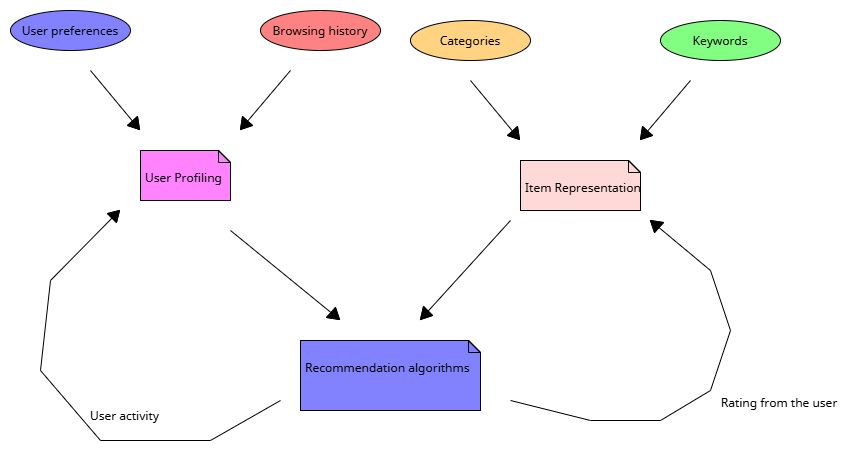
\includegraphics[width=1\linewidth]{Diagram 2.png}
    \caption{How the recommendation system works}
    \label{fig:recommendations}
\end{figure}
 


\newpage
\section{Types of recommendation systems} \label{Types of recommendation systems}

In general, recommendation systems are divided into two types: Collaborative Filtering and Content-Based Filtering\cite{types}.

\begin{enumerate}
\item  \textbf{Collaborative Filtering}

Collaborative filtering relies on the idea that users who agreed in the past will agree in the future. The system finds two people with similar user profiles and recommends to one of them what the other liked, expecting that he will like it too, because they have similar interests.
\begin{figure}[!h]
    \centering
    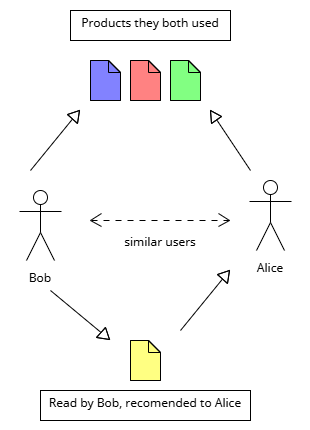
\includegraphics[width=0.8\linewidth]{Diagram 3.png}
    \caption{Collaborative Filtering Diagram}
    \label{fig:collaborative}
\end{figure}

\newpage
\item  \textbf{Content-Based Filtering}

Content-based filtering focuses on the characteristics of the items themselves rather than on user interactions. If the user has chosen items in the past that were somewhat similar to each other, the system will recommend things that also have something in common with them, expecting the user to like it because he liked it in the past.
\begin{figure}[!h]
    \centering
    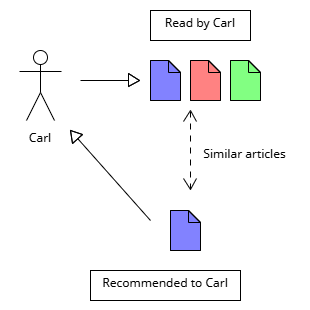
\includegraphics[width=0.7\linewidth]{Diagram 4.png}
    \caption{Content-based Filtering Diagram}
    \label{fig:content-based}
\end{figure}
	

\item  \textbf{Combined}

But the most effective method is to combine these two types. This allows you to create personalized recommendations based on both a person's past actions and the actions of people with similar preferences. Such recommendations are best suited to the user's preferences.

This is proven by the results of this study\cite{user}.

\begin{figure}[!h]
    \centering
    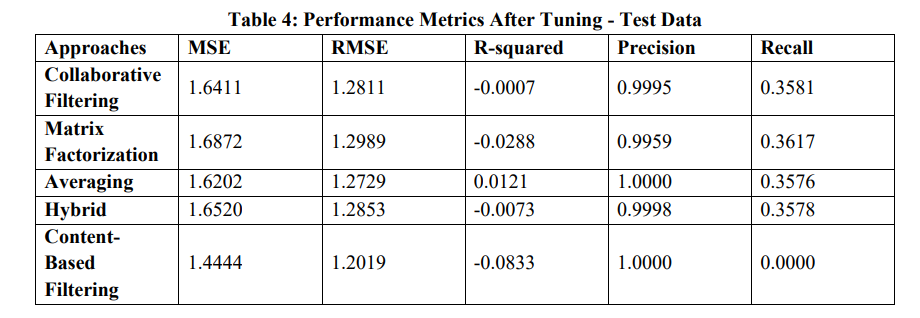
\includegraphics[width=0.87\linewidth]{Table.png}
    \caption{Research}
    \label{fig:research}
\end{figure}

\end{enumerate}


\section{Benefits for Users} \label{Benefits for Users}
Users gain several significant benefits from recommendation systems that enhance their experience with products and services\cite{user}. First, these systems provide personalization by offering recommendations based on user preferences and behavior, helping users find items or content that best match their individual tastes.

Second, thanks to automated recommendations, users can save time by quickly locating what they need without having to sift through a vast amount of information. This makes the process of shopping or searching for content more efficient. Additionally, recommendation systems open up new possibilities by helping users discover products or services they might not have found on their own, including new brands, genres, or categories.


Moreover, personalized recommendations increase user satisfaction, as they boost the likelihood that a user will find something they enjoy, which, in turn, enhances overall enjoyment of the purchase or content consumption. Recommendation systems also reduce information overload by filtering through large amounts of available information, helping users avoid stress when choosing from numerous options.

For example, in this study \cite{closeness}using the following formulas

\begin{eqnarray}
    &&\begin{array}{*{35}{l}}
        s_{\alpha \beta}^{\left(\text{CN}\right)}(t)=\underset{i=0}{\overset{N}{\sum}}\,{{a}_{i\alpha}}(t){{a}_{i\beta}}(t), 
    \end{array}
\end{eqnarray}

\begin{eqnarray}
    &&\begin{array}{*{35}{l}}
        s_{\alpha \beta}^{\left(\text{cosine}\right)}(t)=\frac{1}{\sqrt{{{k}_{\alpha}}{{k}_{\beta}}}}\underset{i=0}{\overset{N}{\sum}}\,{{a}_{i\alpha}}(t){{a}_{i\beta}}(t). 
    \end{array}
\end{eqnarray}

researchers have determined that
sufficiently effective systems can increase the accuracy of recommendations for the buyer several times.
\begin{figure}[!h]
    \centering
    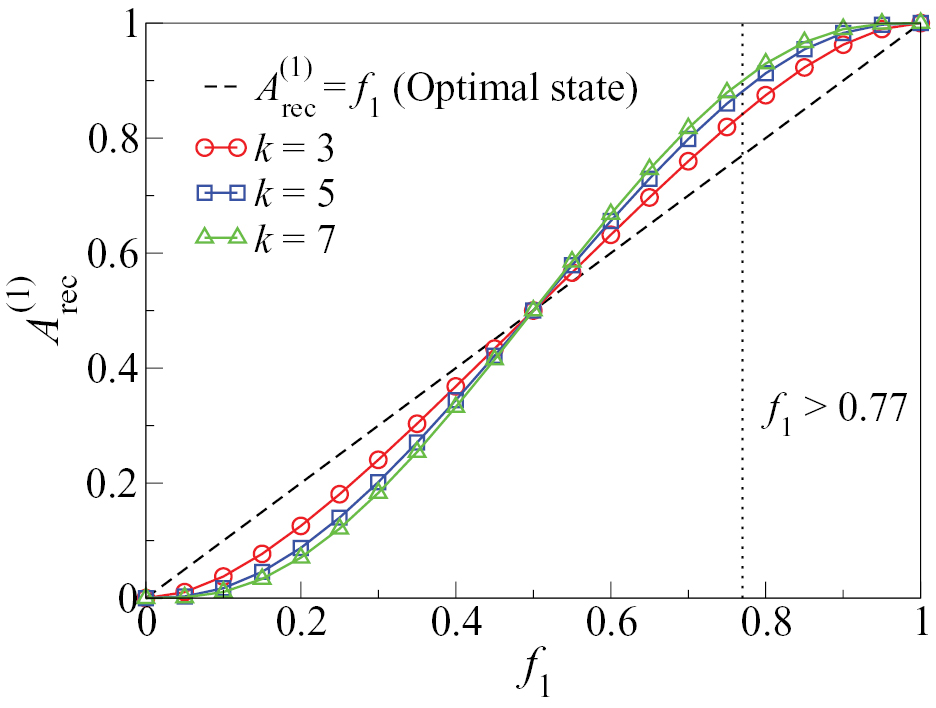
\includegraphics[width=0.9\linewidth]{picture.jpg}
    \caption{closeness of the recommended to the desired result}
    \label{fig:closeness}
\end{figure}

Furthermore, users who receive relevant recommendations are more likely to engage with the platform, which can lead to repeat purchases or more frequent use of services. In some systems, the opinions of friends or other users are taken into account, allowing for recommendations based on social connections and increasing trust in specific products or services.

Finally, recommendation systems can adapt to changes in user preferences by incorporating new data and feedback, ensuring that recommendations remain relevant. In summary, recommendation systems create a more convenient, efficient, and satisfying experience for users, allowing them to find what truly aligns with their interests and needs.




\section{Benefits for Platforms} \label{Benefits for Platforms}
Companies gain numerous advantages from implementing recommendation systems\cite{comerce}, which can significantly enhance their business performance. First and foremost, these systems contribute to increased sales by suggesting relevant products that users may want to purchase, stimulating impulse buys and raising the average transaction value.

Additionally, personalized recommendations improve overall customer satisfaction\cite{user}, leading to a higher level of customer contentment. Satisfied customers are more likely to return and recommend the company to others, fostering positive word-of-mouth. Moreover, when users receive tailored suggestions that align with their interests, the likelihood of cart abandonment decreases, which is especially crucial in a competitive market.

Recommendation systems also help build customer loyalty by creating a closer connection between users and the brand\cite{user}. When a company offers relevant content or products, it fosters brand loyalty among its customers. Furthermore, the data analyzed by these systems provides valuable insights into customer behavior and preferences, allowing companies to refine their marketing strategies effectively.

By enabling more precise targeting in marketing campaigns, recommendation systems can optimize marketing expenditures, reducing costs while increasing effectiveness\cite{comerce}. Recommendations based on user interests can lead to higher conversion rates, making marketing efforts more efficient\cite{user}.

Moreover, companies that successfully implement effective recommendation systems can gain a competitive edge in the market by offering a more personalized experience compared to their rivals\cite{comerce}. This competitive advantage can be crucial in attracting and retaining customers.

Finally, personalized recommendations can encourage users to spend more time on the platform\cite{experience}, which may lead to increased purchases or content consumption. In summary, recommendation systems not only enhance user experience but also provide substantial business benefits, such as increased sales, reduced marketing costs, and strengthened customer loyalty. Implementing such systems is becoming an essential element of successful business strategy in today’s competitive environment.


\newpage
\section{Ethical and Legal Issues} \label{Ethical and Legal Issues}
\begin{itemize}



\item \textbf{Data Privacy and Consent} 

One of the primary ethical issues surrounding recommendation systems is the collection and use of personal data\cite{problems}. These systems often rely on vast amounts of user information, including browsing history, purchase behavior, and demographic details, to generate tailored recommendations. This raises questions about user consent and the transparency of data usage. Users may not fully understand how their data is being collected, processed, and shared, leading to potential violations of privacy rights.

\item \textbf{Regulatory frameworks}

Regulatory frameworks , such as the General Data Protection Regulation (GDPR) in the European Union, have been established to address these concerns. These regulations mandate that organizations obtain explicit consent from users before collecting their data and provide them with the right to access, rectify, or delete their personal information\cite{ethical}. However, compliance can be complex, and many organizations struggle to navigate these legal requirements effectively.


\item \textbf{Algorithmic Bias and Fairness} 

Another critical ethical issue is algorithmic bias\cite{problems}, which can arise when recommendation systems inadvertently reinforce existing stereotypes or discrimination. If the data used to train these systems is biased—reflecting historical inequities—this can result in skewed recommendations that perpetuate harmful social dynamics. For instance, a system might recommend products primarily to certain demographic groups while neglecting others, thus limiting diversity and inclusion in content and offerings.

To mitigate these biases, it is essential for developers to implement fair algorithms and continuously evaluate their performance across different user groups. This involves diverse data collection practices and regular audits to identify and rectify any biases in the recommendation process.

\item \textbf{Manipulation and User Autonomy} 

Recommendation systems also raise concerns about manipulation and the erosion of user autonomy\cite{problems}. By presenting content that aligns with a user’s past preferences, these systems can create "echo chambers," where individuals are only exposed to viewpoints and products that reinforce their existing beliefs. This can limit exposure to diverse perspectives and contribute to polarization in society.


\item \textbf{Intellectual Property and Content Ownership} 

The use of recommendation systems also intersects with legal issues regarding intellectual property and content ownership\cite{ethical}. When these systems aggregate and suggest content from various sources, they must navigate copyright laws to avoid infringing on the rights of content creators. Platforms that fail to adequately manage these rights may face legal challenges, necessitating a careful approach to how they curate and present content.

\newpage
\item \textbf{Conclusion} 

In conclusion, while recommendation systems offer significant benefits in enhancing user experience and driving sales, they also pose considerable ethical and legal challenges. Organizations must prioritize transparency, fairness, and user consent in their data practices, actively work to mitigate bias, and ensure that their systems foster informed choices rather than manipulation. By addressing these issues proactively, companies can build trust with their users and contribute to a more ethical digital landscape.

\end{itemize}



\section{Risks of Data Breaches} \label{Risks of Data Breaches}

One of the primary risks is the exposure of personal data. These systems collect sensitive information, including user preferences and behavior patterns\cite{info}. A data breach can lead to unauthorized access, putting users at risk of identity theft and fraud. This potential for personal data exposure is compounded by the fact that users may feel vulnerable and less inclined to share information, which can lead to a decline in user engagement and loyalty.

The loss of trust is another critical consequence of data breaches. When users learn that their data has been compromised, their confidence in the platform diminishes\cite{data}. Rebuilding this trust can be a challenging and lengthy process, often requiring significant investments in public relations and enhanced security measures.


Moreover, the algorithms and data processing techniques used in recommendation systems represent substantial intellectual property for companies. A breach may expose these proprietary elements to competitors, potentially undermining the original company's market position and innovation.

Regulatory consequences are also a pressing concern. With regulations like GDPR and CCPA in effect, organizations face severe penalties for failing to protect user data. A data breach could lead to hefty fines and increased scrutiny from regulatory bodies, complicating future business operations.

Operational disruption is another risk associated with data breaches\cite{info}. Such incidents can lead to downtime and affect the overall availability of services, resulting in immediate financial losses and long-term damage to brand reputation. Additionally, if attackers gain access to recommendation systems, they could manipulate the algorithms to serve misleading or harmful content, further endangering users and tarnishing the company’s image.

Finally, a successful data breach can expose vulnerabilities within an organization’s security infrastructure\cite{data}. This may lead to repeated attacks, compounding the damage over time and creating a cycle of security failures.

In conclusion, while recommendation systems offer valuable benefits, the risks associated with data breaches must be taken seriously. Organizations should prioritize robust security measures, conduct regular audits, and foster a culture of data protection. By safeguarding user data, companies can enhance trust, protect their intellectual property, and ensure compliance with regulatory standards, ultimately leading to a more secure and reliable user experience.


\newpage
\section{Information Bubbles} \label{Information Bubbles}
\begin{itemize}

\item \textbf{What Are Information Bubbles?} 

Information bubbles occur when users are exposed predominantly to viewpoints and content that align with their existing beliefs and preferences, while alternative perspectives are minimized or excluded\cite{boubble}. This phenomenon is often amplified by recommendation algorithms that prioritize content similar to what users have previously engaged with, leading to a narrow range of exposure.

\item \textbf{The Mechanism of Information Bubble} 

Recommendation systems analyze user behavior—such as clicks, likes, and shares—to predict what content users are likely to engage with next\cite{boubble}. While this personalization can enhance user experience, it often results in a feedback loop where users are continually fed similar content\cite{trouble}. For example, a user who frequently watches political commentary from a specific viewpoint may find their feed increasingly filled with similar perspectives, reinforcing their existing beliefs\cite{politics}.

\item \textbf{Consequences of Information Bubbles} 
\begin{enumerate}

\item \textbf{Limited Worldview}

Users may become trapped in a bubble where they only encounter information that confirms their existing beliefs\cite{trouble}. This can lead to a distorted understanding of complex issues and an inability to engage with differing viewpoints.


\item \textbf{Polarization}

Information bubbles can contribute to societal polarization, as individuals become more entrenched in their views and less willing to consider alternative perspectives\cite{politics}. This is particularly concerning in political discourse, where exposure to a single narrative can exacerbate divisions within society.

\item \textbf{Reduced Critical Thinking}

When users are consistently presented with similar ideas, their critical thinking skills may diminish\cite{sssr}. The lack of diverse viewpoints can hinder the ability to analyze and evaluate information effectively.


\item \textbf{Impact on Decision-Making}

Information bubbles can influence important decisions, from consumer choices to voting behavior\cite{politics}. If individuals are only exposed to a narrow range of options or opinions, their decision-making processes may be skewed.

\item \textbf{Undermining Trust in Media}

As users encounter content that aligns with their biases, they may develop mistrust toward sources that present contrasting viewpoints\cite{boubble}. This erosion of trust can further entrench information bubbles and diminish the perceived credibility of diverse media.
\end{enumerate}

\newpage
\item \textbf{Addressing Information Bubbles} 

To mitigate the effects of information bubbles, both users and platforms have roles to play. Users can actively seek out diverse sources of information, engage with different viewpoints, and critically evaluate content. On the other hand, recommendation systems can be designed with greater transparency and accountability, incorporating mechanisms that promote exposure to a broader range of perspectives\cite{youtube}.

Additionally, platforms can implement features that encourage users to explore content outside their usual preferences\cite{youtube}. This could involve presenting alternative viewpoints or highlighting popular content from diverse sources, thereby fostering a more well-rounded information ecosystem.

\item \textbf{Conclusion} 

While recommendation systems provide valuable personalization, they also pose the risk of creating information bubbles that limit users' exposure to diverse viewpoints. Recognizing and addressing these bubbles is crucial for promoting critical thinking, reducing polarization, and fostering a more informed society. By encouraging a broader range of information, we can work towards a more balanced understanding of the world around us.
\end{itemize}

\section{Current and Future Solutions} \label{Current and Future Solutions}

\begin{itemize}



\item \textbf{Hybrid Models} 
One solution to many of the current issues is the use of hybrid models, which combine multiple recommendation techniques (e.g., collaborative filtering, content-based filtering, and knowledge-based methods)\cite{future}. This approach helps overcome the limitations of individual methods, such as data sparsity or cold start problems, by leveraging different types of information\cite{multimodal}. The future of hybrid models lies in integrating deep learning, reinforcement learning, and symbolic reasoning to better handle both explicit and implicit user feedback.


\item \textbf{Transfer Learning and Few-Shot Learning}
Transfer learning, where models trained on one domain are adapted to another, and few-shot learning, which enables learning from a limited amount of data, are promising techniques to solve the cold start problem\cite{future}. These methods can help recommendation systems adapt to new users and items with minimal historical data, improving the overall personalization of recommendations.



\item \textbf{Context-Aware Recommendation Systems} 
Future recommendation systems are likely to become more context-aware, incorporating factors like time of day, location, and even the user's current mood to provide more relevant suggestions\cite{future}. By using multi-modal data (such as location, browsing history, and sentiment analysis), these systems will offer highly personalized and timely recommendations that better align with users' immediate needs.




\item \textbf{Explainable AI for Recommendations} 
With the growing need for transparency in AI systems, explainable AI (XAI) will play a critical role in the future of recommendation systems\cite{XAI}. Techniques like LIME (Local Interpretable Model-Agnostic Explanations) and SHAP (Shapley Additive Explanations) are already being applied to make complex models more interpretable. In the future, users will be able to understand the reasons behind recommendations, which can improve trust and user satisfaction.



\item \textbf{Multi modal Recommendations} 
The future of recommendation systems will involve multimodal approaches that combine different types of data (e.g., text, images, videos)\cite{multimodal}. Cross-domain recommendations, which integrate data from various sources like social media, e-commerce, and entertainment platforms, will offer richer, more comprehensive user profiles and improve the relevance of recommendations.


\item \textbf{Deep Learning for Complex Data} 
Deep learning, particularly convolutional neural networks (CNNs)\cite{CNN} and recurrent neural networks (RNNs)\cite{RNN}, will continue to advance the capabilities of recommendation systems. These models can handle more complex data, such as images, audio, and sequential patterns, allowing for more nuanced recommendations based on user behavior and preferences.


\end{itemize}





\section{Conclusion} \label{Conclusion}

Recommendation systems are used in almost all companies. The amount of money invested in them is growing every year, as can be seen in the following table.


\begin{table}[ht]
\centering
    \begin{tabular}{l|r}
        Year  & Billions of USD \\\hline
        2022  & 2.18   \\
        2023  & 2.80   \\
        2024  & 3.60   \\
        2025  & 4.63   \\
        2026  & 5.94   \\
        2027  & 7.64   \\
        2028  & 9.81   \\
        2029  & 12.61  \\
        2030  & 16.21  \\
        2031  & 20.82  \\
        2032  & 26.76  \\
        2033  & 34.39  \\
    \end{tabular}
    \caption{Finances to be invested in recommendation systems}
    \label{tab:widgets}
\end{table}

These systems play an important role for both companies and customers, so it is hard to imagine the modern world without them. However, they also have a number of drawbacks that have not yet been solved. However, a large number of specialists are currently working on fixing these problems, so even now there are many ways to reduce the negative impact of recommendation systems. In this article, I looked at the general principles of recommendation systems, their types, the problems that arise from their use, and current and future solutions.



\newpage
\bibliography{literatura}
\bibliographystyle{plain}
\end{document}
